\documentclass{article}
\usepackage[utf8]{inputenc}
\usepackage{biblatex}
\usepackage{graphicx}
\usepackage[font=small, labelfont=bf]{caption}
\usepackage{amsmath}
\usepackage{amsthm}
\usepackage{amsfonts}
\usepackage{mathabx}
\usepackage{tikz}
\usepackage{esvect}
\usepackage{changepage}
\usetikzlibrary{automata, positioning, arrows}

\title{Computability, its Proof by Construction, and the Halting Problem}
\author{Oluwafunke Alliyu, Ethan Balcik, Paul John Balderston, Sen Zhu}
\date{April 2021}

\begin{document}
\theoremstyle{definition}
\newtheorem{exmp}{Example}[section]
\newtheorem{defin}{Definition}[section]
\newtheorem{prf}{Proof}[section]

\maketitle

\section{Introduction}
In the age of digital communications, it is difficult to imagine how, in a world without digital computers, one might work toward the development of one.  As a result, often overlooked are the initial developments which led to today's digital age.  Nevertheless, the emergence of digital computers would not be possible without initial, groundbreaking developments in mathematical logic and information theory from significant engineers and mathematicians like Alan Turing and Claude Shannon.  Throughout this paper, we discuss computability in a rigorous, self-contained manner - both its proof by construction and its disproof by contradiction, with examples of each.  Furthermore, we aim to provide our readers with some historical insight into the development of these methods in order to build both an appreciation of their significance, and of the current challenges researchers face as attempts are made to further progress in theoretical computer science \cite{1}.

\section{Background}
Here we introduce the background section
\subsection{Historical Background}
Here we discuss the history behind computer science and its foundations in mathematics
\subsection{Mathematical Logic and Set Theory}
Here we discuss relevant concepts in mathematical logic and set theory
\subsection{Finite State Machines}
Here we discuss finite state machines, state diagrams, etc. to provide the necessary background to understand conceptual machines and understand Turing Machinces graphically

\section{Turing Machines}
An effective model for the general-purpose computer is the Turing Machine, developed by Alan Turing in 1936 \cite{2}.  The Turing Machine is a conceptual model of a general-purpose computing machine which involves the following conceptual components:
\begin{itemize}
	\item A "control box" which stores a finitely-large program
	\item A tape with infinite spaces in which symbols can be stored, read, and written
	\item A read-write mechanism for the tape \cite{3}
\end{itemize}
\begin{figure}[h]
	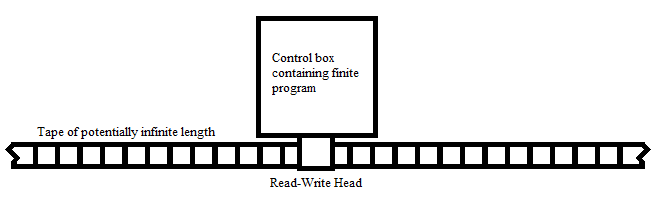
\includegraphics[width=0.85\textwidth]{figure-3-1}
	\centering
	\setlength{\belowcaptionskip}{-10pt}
	\caption{A simple visualization of a Turing machine.  Note that spaces along the tape would be filled with symbols which can be read and written using the read-write head on the machine.}
\end{figure}
\begin{defin}
	A \textbf{Turing Machine} is a 7-Tuple, $(Q, \Sigma, \Gamma, \delta, q_{0}, q_{accept}, q_{reject})$, where:
\end{defin}
\begin{itemize}
	\item $Q$ is a finite set containing the states of the machine
	\item $\Sigma$ is a finite set containing the machine's \textbf{input alphabet}
	\item $\Gamma$ is the finite set containing th emachine's \textbf{tape alphabet} such that the \textbf{blank symbol} $\textvisiblespace \in \Gamma$ and $\Sigma \subseteq \Gamma$
	\item $\delta$ is the \textbf{transition function} $\delta: Q \times \Gamma \to Q \times \Gamma \times \{L, R\}$
	\item $q_{0}$ is the \textbf{starting state} $q_{0} \in Q$
	\item $q_{accept}$ is the \textbf{accept state} $q_{accept} \in Q$
	\item $q_{reject}$ is the \textbf{reject state} $q_{reject} \in Q$ such that $q_{reject} \neq q_{accept}$
\end{itemize}
\noindent A \textbf{configuration} represents the state of a Turing machine's read-write head along its tape, as well as the characters on the tape.  For feasibly-sized tape inputs, a configuration is given as a string of the tape's characters listed starting from the left-most character and working right, with the state $q_{n} \in Q$ inserted to the left of the character currently being read by the read-write head of the machine.  To exemplify this, we can introduce a new instance of a Turing Machine with a specific input, and an algorithm running on the input.
\begin{exmp}
Let's imagine a Turing machine running an algorithm which verifies whether or not a binary string of length $n$ has an even weight (number of 1s in the binary string).  It might achieve this by running the following algorithm:
\begin{enumerate}
	\item Read each bit from left to right on the input string and cross off every other '1' character.
	\item If in step 1 the tape contained no '1' characters, accept.
	\item If in step 1 the tape contained a single '1' character, reject.
	\item Return to the left-most character on the tape.
	\item Return to step 1.
\end{enumerate}
\noindent This particular Turing machine can be given formally as $M = (Q, \Sigma, \Gamma, \delta, q_{1}, q_{accept}, q_{reject})$ such that:
\begin{itemize}
	\item $Q \coloneq \{ q_{1}, q_{2}, q_{3}, q_{4}, q_{5}, q_{accept}, q_{reject} \}$
	\item $\Sigma \coloneq \{ 0, 1 \}$
	\item $\Gamma \coloneq \{ 0, 1, x, \textvisiblespace \}$
	\item The transition function $\delta$ is given as a state diagram (see figure 2)
\end{itemize}
\begin{figure}[h]
	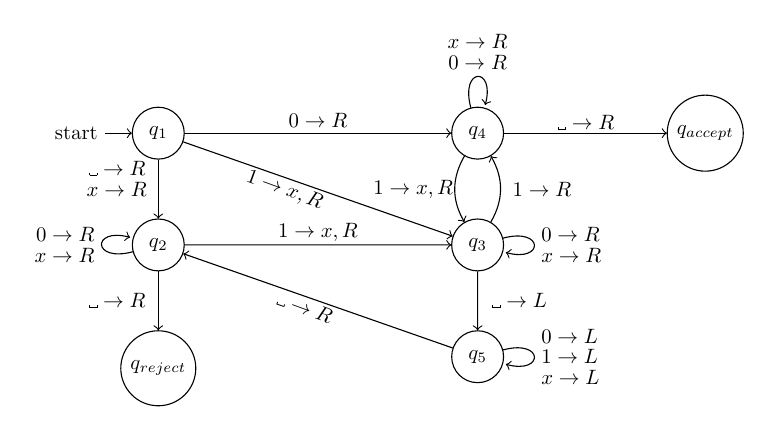
\begin{tikzpicture}[scale=0.75, transform shape]
		\node[state, initial] (q1) {$q_{1}$};
		\node[state, below=of q1] (q2) {$q_{2}$};
		\node[state, right=of q2, xshift=100] (q3) {$q_{3}$};
		\node[state, right=of q1, xshift=100] (q4) {$q_{4}$};
		\node[state, below=of q3] (q5) {$q_{5}$};
		\node[state, below=of q2] (qreject) {$q_{reject}$};
		\node[state, right=of q4, xshift=50] (qaccept) {$q_{accept}$};
		\draw[->] (q1) edge node[yshift=10, xshift=-20] {\tt $\textvisiblespace \rightarrow R$} node[xshift=-20] {\tt $x \rightarrow R$} (q2);
		\draw[->] (q1) edge node[yshift=6] {\tt $0 \rightarrow R$} (q4);
		\draw[->] (q1) edge node[rotate=-20, yshift=-6, xshift=-15] {\tt $1 \rightarrow x , R$} (q3);
		\draw[->] (q2) edge[loop left] node[yshift=5] {\tt $0 \rightarrow R$} node[yshift=-5] {\tt $x \rightarrow R$}(q2);
		\draw[->] (q2) edge node[yshift=6] {\tt $1 \rightarrow x , R$} (q3);
		\draw[->] (q2) edge node[xshift=-20] {\tt $\textvisiblespace \rightarrow R$} (qreject);
		\draw[->] (q3) edge[loop right] node[yshift=5] {\tt $0 \rightarrow R$} node[yshift=-5] {\tt $x \rightarrow R$} (q3);
		\draw[->] (q3) edge[bend right] node[xshift=20] {\tt $1 \rightarrow R$} (q4);
		\draw[->] (q3) edge node[xshift=20] {\tt $\textvisiblespace \rightarrow L$} (q5);
		\draw[->] (q4) edge[bend right] node[xshift=-20] {\tt $1 \rightarrow x , R$} (q3);
		\draw[->] (q4) edge[loop above] node[yshift=10] {\tt $x \rightarrow R$} node {\tt $0 \rightarrow R$} (q4);
		\draw[->] (q4) edge node[yshift=5] {\tt $\textvisiblespace \rightarrow R$} (qaccept);
		\draw[->] (q5) edge node[rotate=-20, yshift=-5, xshift=-5] {\tt $\textvisiblespace \rightarrow R$} (q2);
		\draw[->] (q5) edge[loop right] node[yshift=10] {\tt $0 \rightarrow L$} node[yshift=0] {\tt $1 \rightarrow L$} node[yshift=-10] {\tt $x \rightarrow L$} (q5);
	\end{tikzpicture}
	\centering
	\caption{The transition function $\delta$ given as a finite state machine}
\end{figure}
\noindent Using the transition function $\delta$ as given by figure 2, we can show every configuration for a given input string.  For the sake of the example, let's consider the string $\vv{x} = 1101$.  We have the following configurations (read down each column, and then from left to right):
\begin{center}
\begin{tabular}{ c c c c c }
	$q_{1}1101$ & $x1q_{5}0x$ & $xxq_{3}0x$ & $q_{5}xx0x$ & $xx0xq_{2}\textvisiblespace$ \\
	$xq_{3}101$ & $xq_{5}10x$ & $xx0q_{3}x$ & $q_{5}\textvisiblespace xx0x$ & $xx0x\textvisiblespace q_{reject}$ \\
	$x1q_{4}01$ & $q_{5}x10x$ & $xx0xq_{3}\textvisiblespace$ & $q_{2}xx0x$ \\
	$x10q_{4}1$ & $q_{5}\textvisiblespace x10x$ & $xx0q_{5}x$ & $xq_{2}x0x$ \\
	$x10xq_{3}\textvisiblespace$ & $q_{2}x10x$ & $xxq_{5}0x$ & $xxq_{2}0x$ \\
	$x10q_{5}x$ & $xq_{2}10x$ & $xq_{5}x0x$ & $xx0q_{2}x$
\end{tabular}
\end{center}
\noindent We can clearly see that, since our input string has an odd number of '1' characters, our turing machine rejects it, signifying that it does not have an even weight.  Next, let us walk through each configuration of the even-weighted input string $\vv{x} = 1001$.  We have the following configurations:
\begin{center}
\begin{tabular}{ c }
	$q_{1}1001$ \\
	$xq_{3}001$ \\
	$x0q_{3}01$ \\
	$x00q_{3}1$ \\
	$x00xq_{4}\textvisiblespace$ \\
	$x00x\textvisiblespace q_{accept}$
\end{tabular}
\end{center}
\end{exmp}
\noindent Now, since our input string has an even number of '1' characters, our turing machine accepts it. \cite{2}

\section{Proof of Computability by Construction}
The outcomes observed in \textbf{Example 3.1} are rather self-evident in the definition of a Turing machine, as two of its parameters are the accept state $q_{accept}$ and the reject state $q_{reject}$.  If a Turing machine ever reaches either of these states, then its algorithm will terminate.  However, a third potential outcome when running an algorithm using a Turing machine is that the algorithm may never terminate.  It is this possibility, the possibility that a Turing machine may run indefinitely for some input, from which much of the theory of computability emerges.  In this section, we will build the definitions which found the theory of computability, and explore how we may prove that a function is computable.
\begin{defin}
	An \textbf{alphabet} is a finite set of arbitrary characters which can be used in some code or language.
\end{defin}
\noindent For example, the english alphabet (ignoring all punctuation and special characters) may define its alphabet as $A_{english} \coloneq \{ a, b, ... , z \}$
\begin{defin}
	A \textbf{word} $\vv{x}$ is a string of characters, each of which belonging to some alphabet $A$.
\end{defin}
\noindent Following from the previous example, we may construct words of varying lengths using the english alphabet, such as "the", "dog", "was", and "running".  Each character composing each of these words belong to the alphabet $A_{english}$ defined above.
\begin{defin}
	A \textbf{language} $L$ is the set of all possible words $\vv{x} \in L$ of varying length, over some alphabet $A$.
\end{defin}
\noindent Any combination of english characters imaginable will certainly be a member of the language $L_{english}$ which is defined on the alphabet $A_{english}$ mentioned previously.
\begin{defin}
	A language $L$ is \textbf{Turing-decidable} if there exists some Turing machine $M$ such that, for each input word $\vv{x} \in L$, $M$ either accepts or rejects it. \cite{2}
\end{defin}
\noindent The above definitions are those which found much of the theory of computability.  It does so by use of the Church-Turing thesis, and the wealth of empirical evidence backing it, albeit there is no single, rigorous mathematical proof for this thesis.  Essentially, one interpretation of the thesis states that if one wishes to prove that a certain operation is computable, one can do so by constructing a Turing machine which terminates for all possible inputs into that operation \cite{4}.  To display this, we will prove that the binary 'even weight verification' function introduced in \textbf{Example 3.1} is a computable function.
\begin{prf}
	First, let us note that the input alphabet accepted by our Turing machine (its definition given in $\textbf{Example 3.1}$) $\Sigma \coloneq \{ 0, 1 \}$.  This would imply that the \textbf{language} $L$ emergent from this alphabet is simply the set of all binary strings (or \textbf{words}) of arbitrary length $n \geq 1$.  Thus, our input language can be enumerated using $\mathbb{N}^{2}$.  We must use $\mathbb{N}^{2}$ as opposed to simply $\mathbb{N}$ because we note that, for example, the strings $\vv{y}=000101$ and $\vv{z}=101$ are different inputs entirely, and will be handled differently by our Turing machine, even though their decimal values are identical.  Therefore, we allow one degree of freedom to represent the length of the arbitrary input word $\vv{x}$, and the other to represent the decimal value of the arbitrary input word $\vv{x}$.  Using this fact, we can partition our input language into four unique subsets, and engage in a 'proof by cases' on an arbitrary member of each such subset.\\
\begin{adjustwidth}{0.5cm}{}
	\textbf{Case 1:} Let $\vv{x} \in L$ be an arbitrary-length input string with even weight, and starting with the '0' character.  Our Turing machine will begin in state $q_{4}$.  Since we know that there are an even number of '1' characters in $\vv{x}$, we can expect our Turing machine to 'bounce' back and forth between states $q_{4}$ and $q_{3}$ an even number of times, crossing off every other '1' character with an 'x' character, until ultimately producing some configuration $\dots q_{4}\textvisiblespace$.  This will finally yield the configuration $\dots \textvisiblespace q_{accept}$, and the Turing machine will terminate in state $q_{accept}$ as expected.\\
\end{adjustwidth}
\begin{adjustwidth}{0.5cm}{}
	\textbf{Case 2:} Let $\vv{x} \in L$ be an arbitrary-length input string with even weight, and starting with the '1' character.  Our Turing machine will begin in state $q_{3}$ with the first '1' character crossed off.  Since we know that there are an even number of '1' characters, and that we have already crossed off one of these characters, we can expect our Turing machine to 'bounce' back and forth between states $q_{3}$ and $q_{4}$ an odd number of times, crossing off every other '1' character with an 'x' character.  Ultimately, this will produce the configuration $\dots q_{4}\textvisiblespace$, which will finally yield the configuration $\dots \textvisiblespace q_{accept}$, and the Turing machine will terminate in state $q_{accept}$ as expected.\\
\end{adjustwidth}
\begin{adjustwidth}{0.5cm}{}
	\textbf{Case 3:} Let $\vv{x} \in L$ be an arbitrary-length input string with an odd number of '1' characters, and starting with the '1' character.  Our Turing machine will begin in state $q_{3}$ with the first '1' character crossed off.  Since we know that there are an odd number of '1' characters, and that we have already crossed off one of these characters, we can expect our Turing machine to 'bounce' back and forth between states $q_{3}$ and $q_{4}$ an even number of times, crossing off every other '1' character with an 'x' character.  Ultimately, this will produce the configuration $\dots q_{3}\textvisiblespace$, which will trigger the $q_{5}$ state, eventually returning the system to the $q_{2}$ state with the read-write head reading the first character of the string.  Note that, since the input string had an odd weight, but had the first '1' character crossed off before the initial loop between states $q_{3}$ and $q_{4}$, it now has an odd number of '1' characters crossed off, and thus, an even number of '1' characters remaining.  From here, the machine will proceed with this process recursively until it crosses off all '1' characters, and is left with the configuration $q_{2} \dots$, where $q_{2}$ will inevitably sweep through the entire string, producing the configuration $\dots q_{2} \textvisiblespace$.  As a result, the Turing machine will transition to the configuration $\dots \textvisiblespace q_{reject}$ as expected for our odd-weighted input string.\\
\end{adjustwidth}
\begin{adjustwidth}{0.5cm}{}
	\textbf{Case 4:} Let $\vv{x} \in L$ be an arbitrary-length input string with odd weight, and starting with the '0' character.  Our Turing machine will begin in state $q_{4}$.  Since we know that there are an odd number of '1' characters, we can expect our Turing machine to 'bounce' back and forth between states $q_{4}$ and $q_{3}$, crossing off every other '1' character with an 'x' character.  Ultimately, this will produce the configuration $\dots q_{3}\textvisiblespace$, which will trigger the $q_{5}$ state, eventually returning the system to the $q_{2}$ state with the read-write head reading the first character of the string.  Note that, since the input string had an odd weight, and since the transition between $q_{4}$ and $q_{3}$ took place an odd number of times starting with $q_{4}$, then in the current state with $q_{2}$ back at the beginning of the input string, we have the original input string, but with an odd number of '1' characters crossed off, and thus, an even number of '1' characters remaining.  From here, our Turing machine will engage in an identical recursive process as given in \textbf{case 3}, meaning that it will terminate in state $q_{reject}$ as expected.\\
\end{adjustwidth}
Terefore, the binary 'even weight verification' function is computable, as it terminates for all input words $\vv{x} \in L$. \qedsymbol
\end{prf}

\section{The Halting Problem}
Alan Turing, during the 20th century, used similar concepts from computability theory to prove that first-order logic is, in fact, non-decidable.  This was a major question in the field of mathematical logic for some time, and Turing was among one of the first to prove this fact.  In order to prove this fact, Turing showed that there exists no finite program which terminates for every possible input belonging to the language of first-order logic.  The proof that Turing constructed is known commonly as \textbf{the halting problem}, and it goes as follows. \cite{7}
\begin{prf}
	Assume there exists some program $M$ which accepts as its input parameters a program $P$, and a particular input for $P$ which we'll call $I$.  Assume that $M$ determines whether $P$ terminates for the input $I$, itself terminating in state $q_{accept}$ if $P$ terminates for the input $I$, and terminating in state $q_{reject}$ if not.  Finally, and most importantly as we work toward a contradiction, assume that $M$ itself terminates for all possible inputs $P$ and $I$.  To begin the proof, we generate a new Turing machine by transforming $M$ in such a way that simple logic is appended to the end of $M$'s program.  We say that, if the new Turing machine, which we'll call $M'$, enters state $q_{accept}$, it should loop forever, and if $M'$ enters state $q_{reject}$, then it should terminate in state $q_{accept}$.  We now feed $M'$ into itself with $M'$ as its input.\\
\begin{adjustwidth}{0.5cm}{}
	\textbf{Case 1:} If we assume the program $M'$ terminates on input $M'$, then $M'$ will loop forever, leading to a contradiction.\\
\end{adjustwidth}
\begin{adjustwidth}{0.5cm}{}
	\textbf{Case 2:} If we assume the program $M'$ loops forever on input $M'$, then $M'$ will terminate, also leading to a contradiction.\\
\end{adjustwidth}
	\noindent Therefore, if we assume that there exists some program $M$ which determines whether an input program given its input terminates, then we are led to a contradiction in both cases. \cite{5} \qedsymbol
\end{prf}

\section{Conclusions}
Here we finally discuss the conclusions of the paper

\begin{thebibliography}{100}
	\bibitem{1} National Research Council. (1999). Funding a Revolution: Government Support for Computing Research. Washington, DC: The National Academies Press. https://doi.org/10.17226/6323.
	\bibitem{2} Sipser, Michael. (2013). Introduction to the Theory of Computation. Cengage Learning. Third Edition. Print.
	\bibitem{3} Mainzer, Klaus. (2018). Proof of Computation: Digitization in Mathematics, Computer Science, and Philosophy. World Scientific. https://doi.org/10.1142/11005
	\bibitem{4} Evans, David. (2010). Church-Turing Thesis. University of Virginia. Web. http://www.cs.virginia.edu/~evans/cs3102-s10/classes/class15/class15.pdf
	\bibitem{5} Pruhs, Kirk. (1997). Halting Problem - Simple Proof. Web. https://www.comp.nus.edu.sg/~cs5234/FAQ/halt.html
	\bibitem{6} Cornell University. (2012). Introduction to Algorithms: Notes on Turing Machines. Web. http://www.cs.cornell.edu/courses/cs4820/2012sp/handouts/turingm.pdf
	\bibitem{7} Jago, Mark. (2014). Turing and The Halting Problem - Computerphile. YouTube. https://www.youtube.com/watch?v=macM\_MtS\_w4
\end{thebibliography}

\end{document}